\thispagestyle{empty}
\chapter{The mathematics of molecular evolution}
{\hypersetup{linkcolor=GREYDARK}\minitoc}
\label{chap:intro-formalism}

In molecular evolution, the information contained in empirically observed sequences is leveraged to reconstruct ancestral lineages and to unveil the evolutionary mechanisms having generated this diversity of sequences.
In other words, the task is to reconstruct the ancestral path followed by lineages using the knowledge available today, by working backward in time.
To do so, however, requires a theoretical model of the generating process forward in time.
One can then play this model forward in time and relate the resulting generated sequences to empirically observed patterns.

Working out the long-term molecular evolutionary process first requires to formalize what happens in a short time period within populations.
Population genetics, with its assumptions and limitations, provides the theoretical framework for this.
The first section thus recalls the basics of mathematical population genetics, and more specifically, the Wright-Fisher model and its assumptions.
This will allow me to relate parameters of evolution such as mutation, selection and drift to observable patterns in molecular sequences such as the probability of fixation of a mutant \gls{allele}, as well as the expected number of copies of the derived \gls{allele} we should observe in a population.
These relationships between the underlying evolutionary forces and the observable patterns will subsequently be leveraged and recruited in the next section to derive an approximation of the long-term process of sequence \gls{substitution}, again, parameterized directly in terms of mutation, selection and drift.

Although the mathematical proofs for most of the results presented here are out of the scope of this manuscript, an effort was made to state all definitions and assumptions.
Such an effort is meant to clearly define the models, their assumptions and their parameterization from the ground up.


\section{Population genetics of sequences}

\subsection{The Wright-Fisher model}

The Wright-Fisher model describes the change in frequency of a \gls{polymorphic} gene with two \glspl{allele} in a \gls{diploid} population over time.
The population is assumed to consist of fixed number of \gls{diploid} individuals $N \gg 1$.
It is also assumed to be panmictic (i.e.~non-preferential random mating), with non-overlapping generations.
The number of copies of the derived \gls{allele} $B$ present at the current generation is denoted $i$ and the frequency of this mutant \gls{allele} $B$ is denoted $p = i/2N$, while the frequency of the resident $A$ \glspl{allele} is $1 - p$.

The ability to survive and produce offspring differs between the three \gls{diploid} genotypes ($AA$, $AB$, $BB$).
Here, selection is assumed to occur between the zygotic and the adult stage, called post-zygotic selection.
Quantitatively, selection is captured by a measure called Wrightian fitness ($\wrightfit$), which, for a given \gls{diploid} genotype, is defined as the expected number of offspring produced by an individual having this genotype.
Since the population is regulated in size, only the relative fitness matters, which is usually set to $1$ for the reference (wild-type) genotype.
It is convenient to define the fitness of the other two genotypes, relative to the wild-type, in terms of a selection coefficient.
Furthermore, in the following, we will assume additive effects (co-dominance), such that the heterozygote has an intermediate fitness between the two homozygotes.
Altogether, fitness of the three \gls{diploid} genotypes are defined as:
\begin{equation}
    \begin{dcases}
        \wrightfit_{AA} & = 1 \\
        \wrightfit_{AB} & = 1 + s \\
        \wrightfit_{BB} & = 1 + 2s \\
    \end{dcases}
\end{equation}

More generally than the previous equations, under the assumption that selection is weak $|s| \ll 1$, the selection coefficient can be approximated by the difference in Wrightian fitness of the mutant and the resident \gls{allele} as:
\begin{align}
    s & = \dfrac{\wrightfit_{B} - \wrightfit_{A}}{\wrightfit_{A}}, \\
    & = \dfrac{\wrightfit_{B}}{\wrightfit_{A}} - 1, \\
    & \simeq \ln\left( \dfrac{\wrightfit_{B}}{\wrightfit_{A}} \right), \\
    & \simeq \ln(\wrightfit_{B}) - \ln(\wrightfit_{A}), \\
    & \simeq \logfit_{B} - \logfit_{A},
\end{align}
where $f = \ln(\wrightfit)$ is often referred to as the Malthusian fitness, relative fitness or also log-fitness.

\subsection{Frequency changes across successive generations}

Under the Hardy-Weinberg equilibrium of the population, the \gls{diploid} genotype frequencies in the current generation are distributed as given in table~\ref{table:fitnesses}.

As a result, the mean fitness in the population is a function of the selection coefficient and the frequency of two \glspl{allele} as:
\begin{align}
    \overline{\wrightfit} &= (1+2s)p^2 + (1+s)2p(1-p) + (1-p)^2 \\
    &= 1 + 2ps,
\end{align}
And the relative fitness of the three different genotypes are also shown in table~\ref{table:fitnesses}.

\begin{table}[H]
    \centering
    \noindent\adjustbox{max width=\textwidth}{%
    \begin{tabu}{|l||c|c|c|}
        \hline
        \textbf{Genotype} & $AA$ & $AB$ & $BB$ \\
        \hline
        \textbf{Wrightian fitness ($\bm{\wrightfit}$)}  & $1$ & $1+s$ & $1+2s$ \\
        \hline \textbf{Hardy-Weinberg frequency}  & $(1-p)^2$ & $2p(1-p)$ & $p^2$\\
        \hline \textbf{Relative Wrightian fitness}  & $\dfrac{1}{1+2ps}$ & $\dfrac{1+s}{1+2ps}$ & $\dfrac{1+2s}{1+2ps}$\\
        \hline
    \end{tabu}}
    \caption[Fitnesses of the different genotypes]{Fitnesses of the different genotypes}\label{table:fitnesses}
\end{table}

Reproduction proceeds in two steps.
In a first step, a very large pool of \glspl{gamete} is produced, in which adults contribute proportionally to the fitness of their genotype.
Altogether, the frequency $p'$ of \glspl{gamete} bearing the $B$ \gls{allele} is a function of $p$ and $s$, as shown in figure~\ref{fig:frequency-derived-allele}, and formally derived as:
\begin{align}
    p' & = p^2 \dfrac{1+2s}{1+2ps} + p (1-p)\dfrac{1+s}{1+2ps}\\
    & = p\dfrac{1+s(1+p)}{1 + 2ps}
\end{align}

\begin{figure}[H]
    \centering
    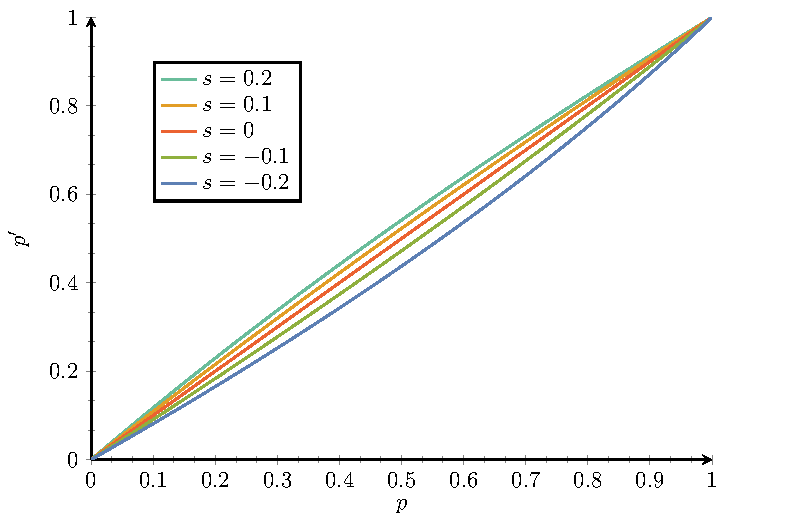
\includegraphics[width=0.8\textwidth, page=1] {figures.pdf}
    \caption[Frequency of derived {allele} after a generation]{
    Frequency of derived \gls{allele} $p'$ after a generation in the vertical axis a function of the frequency in the previous generation $p$ in the horizontal axis, shown for several selection coefficients in coloured solid lines.
    Positive selection coefficients ($s > 0$) result in increased derived \gls{allele} frequency at the next generation, which is intuitively expected.
    The effect is stronger when the derived \gls{allele} frequency is close to $0.5$, intuitively because the poll of both \glspl{allele} must be sufficiently large such that they can be replaced.
    It is worth noting that even for strong selection coefficients ($s=0.2$), completely unrealistic in real population, the difference in frequency from one generation to the next is subtle.}
    \label{fig:frequency-derived-allele}
\end{figure}


In a second step, the $N$ individuals of the next generation are obtained by randomly sampling from the pool of \glspl{gamete}.
As a result, the probability $\proba_{ij}$, that there are $j$ copies of the derived \gls{allele} $B$ present at the next generation, given that there were $i$ copies in the current generation is given by the binomial distribution, with a proportion $p'$ of $B$ \glspl{allele} in \glspl{gamete}:
\begin{align}
    \proba_{ij} & = \binom{2 N}{j} \left( p' \right)^j \left(1 - p' \right)^{2 N -j} \\
    & = \binom{2 N}{j} \left( p\dfrac{1+s(1+p)}{1 + 2ps} \right)^j \left(1 - p\dfrac{1+s(1+p)}{1 + 2ps} \right)^{2 N -j} \label{eq:binomial-WF}
\end{align}

These transition probabilities define a discrete-space and discrete-time Markov process.
It has also been shown to be extremely difficult to explicitly derive formulas for several quantities of evolutionary interest.

Of note, under the assumption that selection is weak $|s| \ll 1$, $p'$ reduces to:
\begin{align}
    p' & \simeq p (1 + s + ps - 2ps) \\
    & = p + sp(1-p) \\
    & = p + \Delta p,
\end{align}
where $\Delta p = sp(1-p)$

Intuitively, fluctuations induced by the binomial sampling (equation~\ref{eq:binomial-WF}) are the underlying cause of random drift.
Quantitatively, the expected frequency change from one adult generation to the next adult generation is:
\begin{equation}
    \E[\Delta p] = s p (1-p).
\end{equation}
The variance of this binomial distribution is given by:
\begin{equation}
    \Var[\Delta p] = \frac{p' (1-p')}{2N}
\end{equation}
Since the change in frequency between two generations is small ($p \simeq p'$), the variance is very close to:
\begin{equation}
    \Var[\Delta p] \simeq \frac{p (1-p)}{2N}
\end{equation}
Thus, the variance induced by random drift is inversely proportional to the population size $N$.
Also, if $s \gg 1/2N$, then $\E[\Delta p] \gg \Var[\Delta p]$, or, in other words, the systematic trend imprinted by selection dominates over drift, describing the strong selection regime.
In contrast, if $s \ll 1 / 2N$, drift dominates over selection, describing the effectively \gls{neutral} regime.

\subsection{Effective population size}

The notion of \gls{effective population size}, called $\Ne$, only appears when we apply a panmictic model to a population that is not, or to a real population.
$\Ne$ was originally defined as \textit{"the number of breeding individuals in an idealized population that would show the same amount of dispersion of \gls{allele} frequencies under random \gls{genetic drift} or the same amount of inbreeding as the population under consideration"}~\citep{wright_evolution_1931}.
For most quantities of interest and most real populations, the census population size $N$ of a real population is usually larger than the \gls{effective population size} $\Ne$.
The same population may have multiple \glspl{effective population size} for different genetic loci, as for example sex chromosomes do not have the same population sizes as autosomes.
For the following development, this idealize population with a single effective population $\Ne$ will be assumed.

\subsection{Probability of fixation}

Starting from an initial frequency, the Wright-Fisher process eventually reaches absorption: the derived \gls{allele} either dies out or invades the population and thus reach fixation.
As the \gls{effective population size} ($\Ne$) approaches infinity (i.e.~$ \Ne \to \infty$), and assuming that the selection coefficient scaled by \gls{effective population size} ($\Ne s $) remains constant, the discrete Markov process defined above can be closely approximated by a continuous-time and continuous-space diffusion process.
The parameters of this process are summarize in table~\ref{table:params-popgen} for readability.

\begin{table}[htbp]
    \centering
    \noindent\adjustbox{max width=\textwidth}{%
    \begin{tabu}{|l|c|c|c|}
        \hline
        \textbf{Parameter} & \textbf{Symbol} & \textbf{Range} \\
        \hline
        \hline Census population size & $N$ & $ [10^2, 10^6]$ \\
        \hline \Gls{effective population size} & $\Ne$ & $ [10^2, 10^6]$ \\
        \hline Absolute Wrightian fitness & $\wrightfit$ & $ \simeq 1 $ \\
        \hline Relative fitness & $f=\ln(\wrightfit)$ & $ \ll 1 $ \\
        \hline Selection coefficient & $s$ & $ |s| \ll 1 $ \\
        \hline Scaled selection coefficient & $S=4 \Ne s$ & Finite (negative or positive) \\
        \hline Mutation rate per generation & $u$ & $[10^{-10}, 10^{-7}]$ per site \\
        \hline Scaled mutation rate & $\theta = 4 \Ne u$ & $[10^{-8}, 10^{-1}]$ per site \\
        \hline
    \end{tabu}}
    \caption[Parameters of population genetics]{Parameters of population genetics}\label{table:params-popgen}
\end{table}

Under this diffusive approximation, a partial differential equation known as the Kolmogorov's backward equation can be used to obtain the fixation probability of the derived \gls{allele}.
Formally, for an \gls{effective population size} $\Ne$, \citet{Kimura1962} derived the probability of fixation ($\pfix(s, \Ne, p)$) of a derived \gls{allele} with selection coefficient $s$ and initial frequency $p$ if the selection coefficient is small ($|s| \ll 1$):
\begin{equation}
    \pfix(s, \Ne, p) = \dfrac{1 - \e^{-4 \Ne p s }}{1 - \e^{-4 \Ne s}}.
\end{equation}

Because $s$ and $\Ne$ are confounded parameters, this probability of fixation is denoted $\pfix(S, p)$, as a function the scaled selection coefficient $S = 4 \Ne s$ and $p$, as shown in figure~\ref{fig:pfix-p}, and formally derived as:
\begin{equation}
    \pfix(S, p) = \dfrac{1 - \e^{- p S }}{1 - \e^{-S}}.
\end{equation}


\begin{figure}[H]
    \centering
    \includegraphics[width=0.8\textwidth, page=3] {figures.pdf}
    \caption[Probability of fixation]{
    Probability of fixation $\pfix(S, p)$ in the vertical axis as a function of the initial frequency $p$ in the horizontal axis, shown for different scaled \gls{effective population size} $S=4 \Ne s$.
    In contrast to changes of frequency during a generation, the probability of fixation is sensitive to very weak selection coefficients ($|s| \ll 1$), as long as the scaled selection coefficient is not negligible ($|S| > 1$).
    Intuitively, selective effects are magnified by population size because the fixation probability is the resultant of the overall trajectory of the \gls{allele}, integrating small effects throughout its lifespan. }
    \label{fig:pfix-p}
\end{figure}

An interesting special case is obtained for a new mutation appearing in the population.
Because it is a single mutant, the initial frequency of the derived \gls{allele} is $p = 1 / 2 \Ne$, and this probability of fixation denoted $\pfix(s, \Ne)$ is given by:
\begin{align}
    \pfix(s, \Ne) & = \dfrac{1 - \e^{-2 s}}{1 - \e^{-4 \Ne s}} \\
    & \simeq  \dfrac{2 s }{1 - \e^{-4 \Ne s}}
\end{align}
The special case of a \gls{neutral} \gls{allele} can be obtained by taking the limit when $s$ goes to $0$.
\begin{align}
    \pfix(0, \Ne) & = \dfrac{1}{2 \Ne}
\end{align}
Altogether, the fixation probability of a selected single mutant relative to the fixation probability of a selectively \gls{neutral} single mutant is given as:
\begin{align}
    \dfrac{\pfix(s, \Ne)}{\pfix(0, \Ne)} & \simeq 2 \Ne \dfrac{2s}{1 - \e^{-S}}, \\
    & \simeq  \dfrac{S}{1 - \e^{-S}}, \label{eq:p-fix}
\end{align}
where this quantity is solely dependent on the scaled selection coefficient $S$.
Such essential result has important consequences, random \gls{genetic drift} and selection are intrinsically confounded factors.
As a an example, increasing population size by a factor of $2$ while reducing the selection coefficient by the same amount leads to the exact same equation, such that they are indistinguishable.
Moreover, the equation have different limits as a function of the selection coefficient:
\begin{gather}
    \begin{cases}
        \lim\limits_{S \to -\infty} \dfrac{S}{1 - \e^{-S}} = -S\e^{S} \\
        \lim\limits_{S \to 0} \dfrac{S}{1 - \e^{-S}} = 1 + \dfrac{S}{2}\\
        \lim\limits_{S \to + \infty} \dfrac{S}{1 - \e^{-S}} = S.
    \end{cases} \label{eq:limits-proba-fix}
\end{gather}
More precisely, the scaled fixation probability has different regimes depending on the value of the scaled selection coefficient, as illustrated in figure~\ref{fig:relative-fixation-probability}.
In the regime of a weak selection coefficient, usually defined as $|S| \ll 1$ or $|s| \ll 1 / \Ne$, known as the drift barrier, the mutant \gls{allele} is behaving mostly as a \gls{neutral} \gls{allele}.

\begin{figure}[H]
    \centering
    \includegraphics[width=0.8\textwidth, page=2] {figures.pdf}
    \caption[Relative fixation probability]{
    Fixation probability of a selected \gls{allele} relative to a \gls{neutral} \gls{allele}, shown in the vertical axis, as function of the scaled selection coefficient $S=4 \Ne s$ in the horizontal axis.
    For a substantial negative scaled selection coefficient ($s \leq -1/\Ne$, red-filled area), the probability of fixation is greatly reduced (by an exponential factor), and the \gls{allele} will not likely reach fixation.
    On the other hand, for a positive scaled selection coefficient ($s \geq 1 / \Ne$, green filled area), the ratio is approximately linear with regard to $S$.
    In between, whenever the absolute value of $s$ is close to $1 / \Ne$ (yellow filled area), the \gls{allele} behaves approximately neutrally.}
    \label{fig:relative-fixation-probability}
\end{figure}

\subsection{Site frequency spectrum}
The probability of fixation of an \gls{allele} can be empirically observable, and in the context of a Wright-Fisher processes it is related to selection and drift.
However, this absorbing fate is not the sole characteristic of the process that relates empirical observable quantities to parameters of the process.
Along the whole trajectory of an \gls{allele}, before fixation or extinction, the probability of this \gls{allele} to be at a certain frequency can be related to its selection coefficient and to the \gls{effective population size}.
More precisely, $g(x) \der x $ is the expected time for which the population frequency of derived \gls{allele} is in the range $(x, x+\der x)$ before eventual absorption, as shown in figure~\ref{fig:expected-time-at-f}, which is derived using the Kolmogorov forward equation as a function of $x$ and $S$:
\begin{align}
    g(x, s, \Ne) & = \dfrac{\left( 1 - \e^{- 2 s }\right) \left( 1 - \e^{-4 \Ne s(1-x)}\right)}{ s (1 - \e^{-4 \Ne s})x(1-x)} \\
    \Rightarrow g(x, S) & \approx \dfrac{2 \left( 1 - \e^{-S(1-x)}\right)}{(1 - \e^{-S})x(1-x)} \label{eq:expected_time}
\end{align}

\begin{figure}[H]
    \centering
    \includegraphics[width=0.8\textwidth, page=4] {figures.pdf}
    \caption[Expected time at a derived frequency]{
    Expected time at a derived frequency $g(x, S)$ in the vertical axis as a function of the frequency $x$, shown for different scaled selection coefficient.
    \Glspl{allele} with a positive selection coefficient can be observed at high frequency, while \glspl{allele} with negative selection coefficients are unlikely to be observed at high frequency.}
    \label{fig:expected-time-at-f}
\end{figure}

This equation is solely valid for a gene with two \glspl{allele}, a configuration which is rarely observed in empirical data since more than two variants of a gene are usually present in the population.
However, it is frequent to observe sites inside a gene sequence for which only two \glspl{allele} are segregating.
This observation led to the development of a site-specific Wright-Fisher process, assuming that each site follows an independent process~\citep{Sawyer1992}.
Strictly speaking, this model considers a collection of independently evolving loci, meaning without linkage.
It provides a good approximation if there is free \gls{recombination} between sites.
Moreover, the collection is considered infinite whereas the total mutation rate across this infinite collection is considered finite.
The assumption of an infinite number of sites is necessary to ensure that each mutation arises at a new site, with a Poisson distribution of total rate $u$ per generation for the whole sequence.

From an empirical perspective, for a sample of $n$ sequences taken in the population, the expected number of sites with $i$ copies of the derived \gls{allele} (with $i$ ranging from $1$ to $n - 1$) is denoted $G(i, n)$.
The collection of all $G(i, n)$ generates what is called a site frequency spectrum (\acrshort{SFS}), which can intuitively be interpreted as the discrete version of the expected time at a derived frequency (equation~\ref{eq:expected_time}), readily available from a sample of sequences from a population.
Given the scaled selection coefficient ($S=4 \Ne s$), and the scaled mutation rate per generation for the whole sequence ($\theta = 4 \Ne u $), each entry of the \acrshort{SFS} is:
\begin{align}
    G(i, n) & = \int_{0}^{1}  2 \Ne u g(x, S) \binom{n}{i} x^{i} (1-x)^{n-i} \der x \\
    & = \theta \int_{0}^{1} \dfrac{1 - \e^{-S(1-x)}}{(1 - \e^{-S})x(1-x)} \binom{n}{i} x^{i} (1-x)^{n-i} \der x \\
    & =  \dfrac{\theta }{1 - \e^{-S}} \binom{n}{i} \int_{0}^{1} \left( 1 - \e^{-S(1-x)} \right) x^{i-1} (1-x)^{n-i-1} \der x
\end{align}

This site frequency spectrum can be confronted to empirical \gls{polymorphic} data in order to estimate the scaled selection coefficient of new mutations.
However, a single selection coefficient for all sites and all mutations is biologically not realistic.
Accordingly, a distribution of selection coefficients across sites is assumed, which is usually modelled as a continuous distribution, known as the distribution of fitness effects of mutations (\acrshort{DFE}).
Mixing over this distribution, the \acrshort{SFS} can then be computed as a function of the underlying \acrshort{DFE}, and can thus be estimated based on empirical data~\citep{eyre-walker_distribution_2006, eyre-walker_estimating_2009}.


\section{Mutation-selection process}
The previous section recalled the Wright-Fisher process of evolution inside a population, relating selection and drift to the diversity of sequences, which empirically requires gene sequences for at least several individuals.
However, modelling sequence evolution between different species along lineages is a different endeavour, in which species are often simplified with a single representative sequence, collapsing the intraspecific diversity.
Under this simplification, the interspecific variability and the evolutionary trajectory of sequences are described by the past history of point \glspl{substitution} along lineages.
The rate at which such \gls{substitution} occurs can nonetheless be decomposed into two mechanisms: their origination through mutation and their final fate of fixation or loss, a modelling approach broadly known as the origin-fixation approximation~\citep{McCandlish2014}, illustrated in figure~\ref{fig:point-process}.
Most importantly, this decomposition of \gls{substitution} events into mutation and fixation events is able to conciliate population genetics and interspecific molecular evolution, where the \gls{substitution} history is parameterized by mutation, selection and drift.
In the field of phylogenetics, the origin-fixation framework is more commonly known as the mutation-selection paradigm, where fixation of an \gls{allele} encompasses the effect of natural selection and drift (which are confounded factors, see equation~\ref{eq:p-fix}), and origination corresponds to mutation.
Since the scope of this manuscript emanates from phylogenetics, I will use the convention mutation-selection terminology hereafter.
Of note, a more general mathematical description of the mutation-selection framework recruiting tools from statistical physics can be found in \citet{Sella2005} and \citet{Mustonen2009}.

\begin{figure}[H]
    \centering
    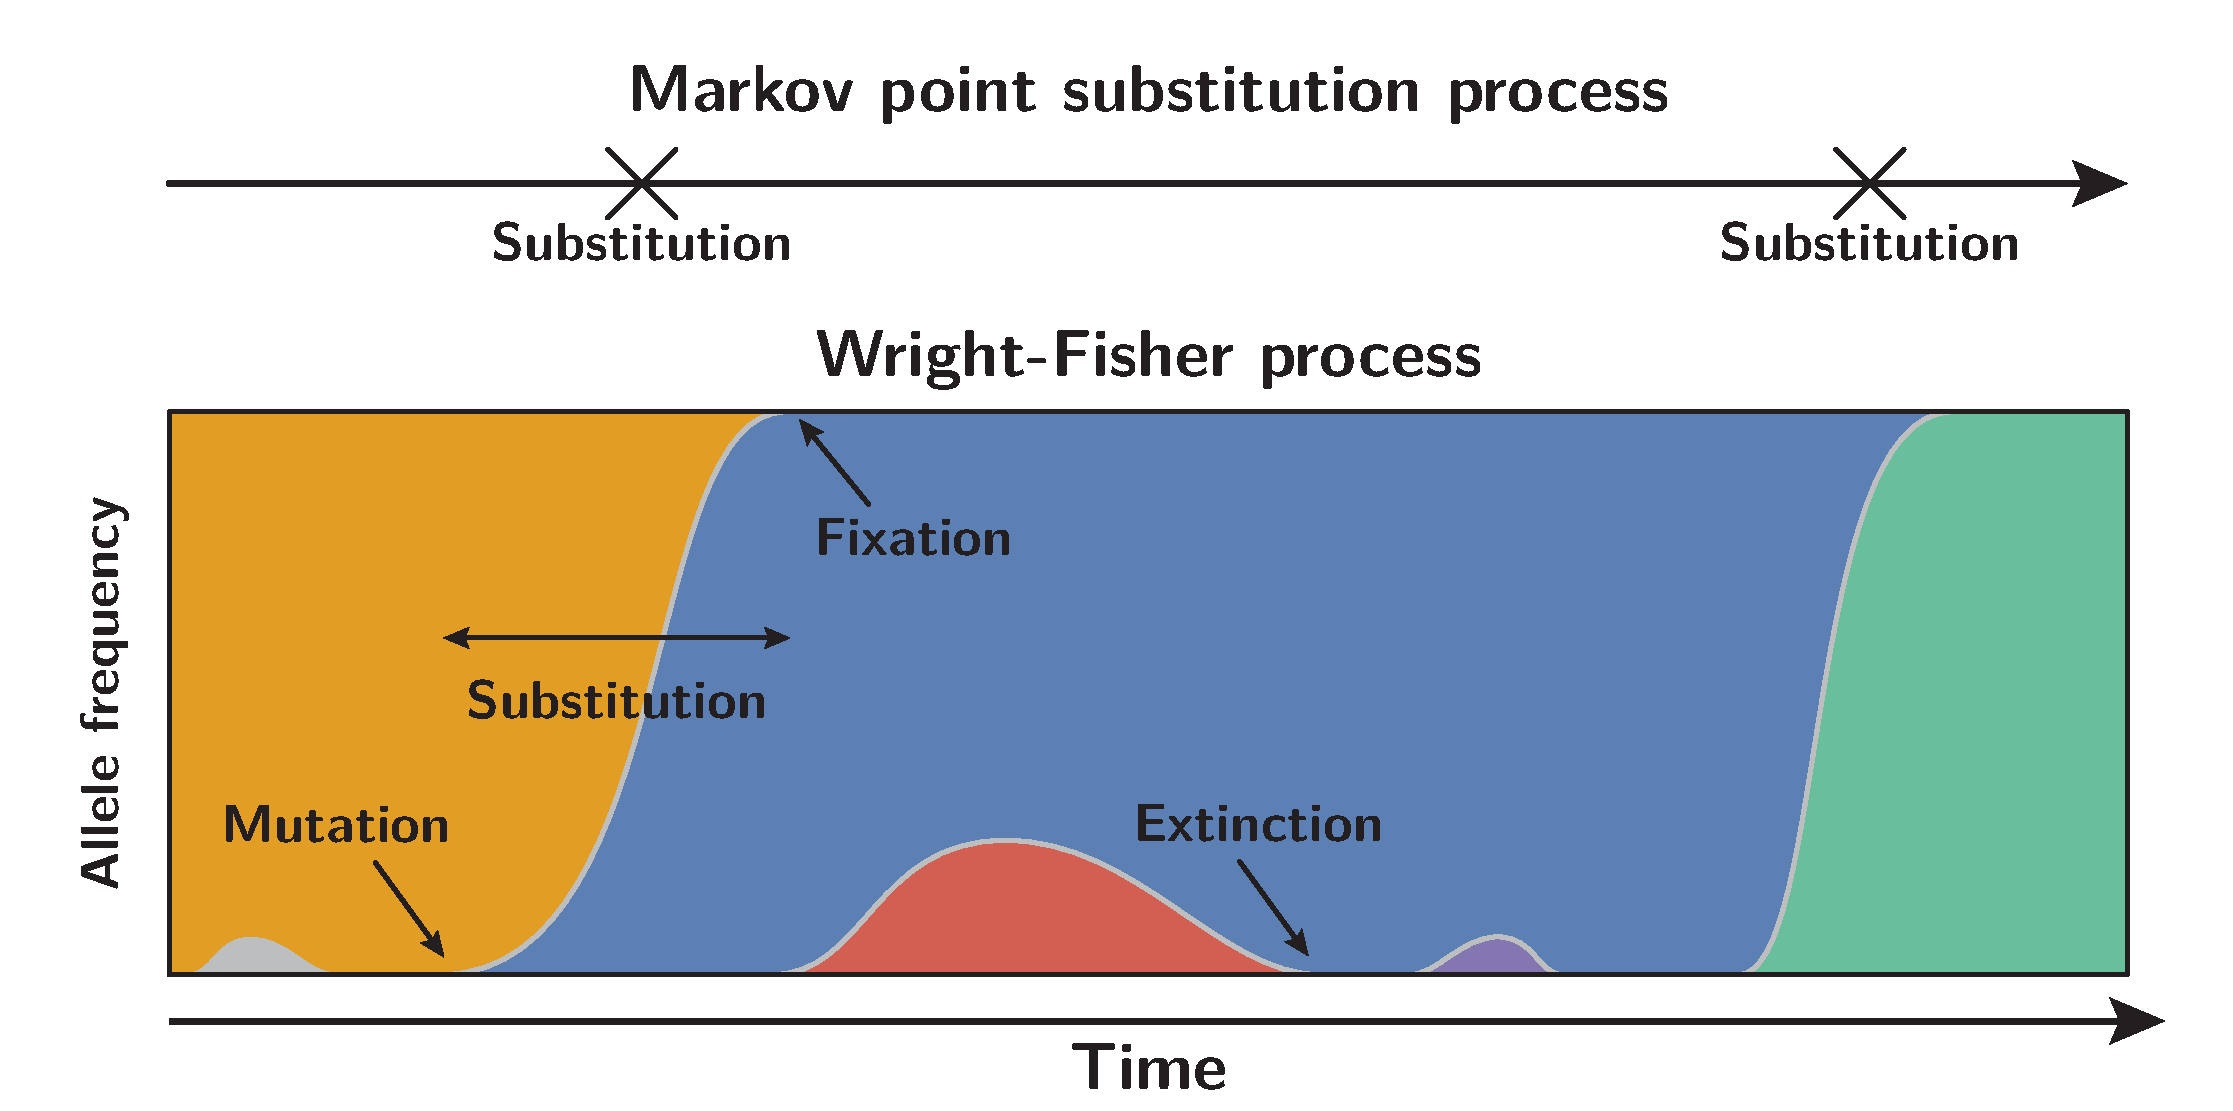
\includegraphics[width=0.75\textwidth]{figures/point-process.pdf}
    \caption[Mutation-selection substitutions models]{
    Mutation-selection \glspl{substitution} models.
    The trajectory of \glspl{allele} inside a population is collapsed into a single point \gls{substitution} process.
    This approximation is valid under low mutation rates such that a mutation originates uniquely whenever the gene is monomorphic (with a single allele).}
    \label{fig:point-process}
\end{figure}

\subsection{Mutation-limited process}
\label{subsec:mutation-limited-assumption}

Mutation-selection probabilistic models are usually Markovian with respect to time, such that the next \gls{substitution} event depends on the current representative sequence but not on earlier sequences visited in the history of a lineage.
This continuous-time Markovian process is valid if the mutation rate is sufficiently low, such that the event of a new mutation reaching fixation is completed before the next one occurs.
Since the rate of \gls{substitution} is equal to $u$ (per generation) and that each \gls{allele} ultimately reaching fixation is segregating for an average of $4 \Ne$ generations~\citep{Kimura1969}, this assumption is broadly applicable whenever the product of population size and mutation rate per generation for the sequence is lower than $1$ ($4 \Ne u \ll 1$).
More strictly, the model would require not only that new mutations reaching fixation do so before the next \gls{substitution} occurs, but before any mutation occurs, even the ones that ultimately become extinct.
Since at each generation during the process an average of $2\Ne$ mutations are produced, the point \gls{substitution} is valid under the condition that $8\Ne^2 u \ll 1$.
In practice, the assumptions that $4 \Ne u \ll 1$ is a sufficient condition for the process to be well approximated.
Throughout this development, it is important to note that $u$ is the mutation rate for the whole sequence under consideration.

For large sequences this approximation is usually not valid, and the sequence is then decomposed into each individual site, forming a collection of independently evolving continuous-time \glspl{Markov chain}.
For such a decomposition to be valid, these models have to assume free \gls{recombination} between sites.
The mutation rate $u$ in this condition then refers to the mutation rate for each independent site, rather than the total mutation rate over the collection as a whole.
For example, \citet{Halpern1998} constructed a model for the evolution of coding sequences where each \gls{codon} site is modelled as an independent \gls{Markov chain}.

\subsection{Substitution rate}
The continuous-time \gls{Markov chain} is defined by the instantaneous rate at which transitions occur between pairs of states.
Parameters of this process are summarized in table~\ref{table:params-mutsel} for readability.

\begin{table}[H]
    \centering
    \noindent\adjustbox{max width=\textwidth}{%
    \begin{tabu}{|l|c|c|c|}
        \hline
        \textbf{Parameter} & \textbf{Symbol} & \textbf{Range} \\
        \hline\hline
        Scaled fitness & $F=4 \Ne f$ & finite, positive or negative \\
        \hline Mutation rate per time & $\mu$ & $[10^{-11}, 10^{-8}]$ per site per year \\
        \hline \Gls{substitution} rate per time & $Q$ & $[10^{-11}, 10^{-8}]$ per site per year \\
        \hline Equilibrium frequency & $\pi$ & $[0, 1]$ \\
        \hline Equilibrium frequency under mutation & $\sigma$ & $[0, 1]$ \\
        \hline Mean scaled fixation probability & $\avgpfix$ & $[0, 1]$ for purifying selection \\
        \hline
    \end{tabu}}
    \caption[Parameters of mutation-selection processes]{Parameter of mutation-selection processes used in this section (\ref{subsec:mutation-limited-assumption})}
    \label{table:params-mutsel}
\end{table}

Given the current state of \gls{allele} $A$, the rate of transition to other states can be derived using the population-genetic equations introduced above.
At each generation, the expectation for the number of possible mutants is $2\Ne u$, and each of these mutants has a probability $\pfix(s, \Ne)$ to result in a \gls{substitution}.
Altogether, the instantaneous rate of \gls{substitution} from \gls{allele} $A$ to $B$, denoted $Q_{A \to B}$, is equal to the rate of mutation ($\mu_{A \to B}$) multiplied by the probability of fixation of the mutation $\pfix(s_{A \to B}, \Ne)$ and scaled by the number of possible mutants at each generation ($2\Ne$):
\begin{align}
    Q_{A \to B} & = 2 \Ne \mu_{A \to B}  \pfix(s_{A \to B}, \Ne) \label{eq:q-pfix}
\end{align}
It is important to note that the \gls{substitution} rate and the mutation rate are in the same units, such that this equation is valid whether the rate is measured either in units of chronological time or per generation (or in branch length, which will matter later on).
As a convention, in what follows, mutation rate is denoted $u$ when measured in units of generation, and denoted $\mu$ when measured in units of time.
As a consequence, $Q$ is measured in units of time in this section.

In the case of selected mutations, the probability of fixation depends on the difference in log-fitness ($\logfit_A$ and $\logfit_B$) between the two \glspl{allele}:
\begin{align}
    Q_{A \to B} & = 2 \Ne \mu_{A \to B} \pfix(s_{A \to B}, \Ne) \\
    & = 2 \Ne \mu_{A \to B}  \dfrac{2(\logfit_{B} - \logfit_{A})}{1 - \e^{4\Ne(\logfit_{A} - \logfit_{B})} } \\
    & = \mu_{A \to B} \dfrac{F_{B} - F_{A}}{1 - \e^{F_{A} - F_{B}} }\text{, where } F = 4\Ne f \label{eq:sub-transion-rates}
\end{align}

In the case of \gls{neutral} mutations, the probability of fixation is independent of the original and target sequence, and equals $1/2 \Ne$.
As a consequence, the \gls{substitution} rate denoted $Q_{A \to B}^{0}$ simplifies to:
\begin{align}
    Q_{A \to B}^{0} & = 2 \Ne \mu_{A \to B}  \pfix(0, \Ne) \\
    & = 2 \Ne \mu_{A \to B} \dfrac{1}{2\Ne} \\
    & = \mu_{A \to B} \label{eq:sub-equal-mut}
\end{align}


If the difference of log-fitness tends to $0$, the \gls{substitution} rate is equal to the mutation rate, retrieving equation~\ref{eq:sub-equal-mut}:
\begin{equation}
    \lim\limits_{|F_{B} - F_{A}| \to 0} Q_{A \to B} =  \mu_{A \to B}
\end{equation}

Taken together, the transition rates which generate the \gls{substitution} history and ultimately the interspecific diversity is parameterized solely by mutation, selection and drift.
Consequently, from a particular history of \glspl{substitution}, one can theoretically estimate the parameters of selection, mutation and drift, although it is important to keep in mind that selection and drift are confounded.


\subsection{Reversibility of the process}
The continuous-time \gls{Markov chain} has so far been defined for $2$ \glspl{allele} but can be generalized to any number of \glspl{allele}, when the number of \glspl{allele} is discrete ($\NbrSites$) and when transition from any \gls{allele} to any other \gls{allele} is possible in one or more \glspl{substitution}.
In this configuration, the transition rates between all possible pairs of \glspl{allele} is defined by equation~\ref{eq:sub-transion-rates}, and equals $0$ whenever single step transitions are not possible.
Because any state is ultimately connected to any other state, the continuous-time \gls{Markov chain} is irreducible.
Moreover, this \gls{substitution} process is positive recurrent and aperiodic since any strictly positive transition rate is matched by a strictly positive transition for the reverse \gls{substitution}.
More precisely, the \gls{substitution} rate between two \glspl{allele} is null only if the underlying mutation rate is null, in which case the transition rate for the reverse mutation is also null, hence the transition rate for the reverse \gls{substitution} is also null.

Theoretically, for an irreducible, positive recurrent and aperiodic continuous-time \gls{Markov chain}, a necessary and sufficient condition to be reversible is given by Kolmogorov's criterion.
Kolmogorov's criterion implies that the product of transition rates through any closed loop is the same whenever the traversing is done forward or in reverse.
As an example for a \gls{Markov chain} composed of $3$ \glspl{allele} ($\ci$, $\cj$ and $\ck$), as illustrated in figure~\ref{fig:reversible-circuit}, the transition rates must satisfy the equality:
\begin{equation}
    Q_{\ci \to \cj}Q_{\cj \to \ck}Q_{\ck \to \ci} = Q_{\ci \to \ck}Q_{\ck \to \cj}Q_{\cj \to \ci}
\end{equation}

\begin{figure}[htbp]
    \centering
    \begin{tikzpicture}[->,>=stealth',auto,node distance=1.2cm and 1.6cm,semithick]
        \tikzstyle{every state}=[]

        \node[] (0) {};
        \node[state] (A) [above=of 0] {$\ci$};
        \node[state] (B) [below left=of 0] {$\cj$};
        \node[state] (C) [below right=of 0] {$\ck$};

        \path[->]
        (A) edge [BLUE,bend right=45] node [left] {$Q_{\ci \to \cj}$} (B)
        (B) edge [BLUE,bend right=45] node [below] {$Q_{\cj \to \ck}$} (C)
        (C) edge [BLUE,bend right=45] node [right] {$Q_{\ck \to \ci}$} (A)
        (B) edge [RED,bend right=15] node [left] {$Q_{\cj \to \ci}$} (A)
        (C) edge [RED,bend right=15] node [below] {$Q_{\ck \to \cj}$} (B)
        (A) edge [RED,bend right=15] node [right] {$Q_{\ci \to \ck}$} (C);
    \end{tikzpicture}
    \caption[Kolmogorov's criterion]{
    The continuous-time \gls{Markov chain} is reversible if the process fulfils Kolmogorov's criterion.
    Namely, the product of the transition rates for a closed loop is equal whether traversed in one sense (blue arrows) or the other (red arrows).}
    \label{fig:reversible-circuit}%
\end{figure}

Kolmogorov's criterion is satisfied under specific conditions for the \gls{substitution} process (\ref{eq:sub-transion-rates}):
\begin{align}
    1 ={}& \dfrac{Q_{\ci \to \cj}Q_{\cj \to \ck}Q_{\ck \to \ci}}{Q_{\ci \to \ck}Q_{\ck \to \cj}Q_{\cj \to \ci}}\\
    ={}& \dfrac{\mu_{\ci \to \cj}\mu_{\cj \to \ck}\mu_{\ck \to \ci}}{\mu_{\ci \to \ck}\mu_{\ck \to \cj}\mu_{\cj \to \ci}} \times \dfrac{(F_{\cj} - F_{\ci})(F_{\ck} - F_{\cj})(F_{\ci} - F_{\ck})}{(F_{\ck} - F_{\ci})(F_{\cj} - F_{\ck})(F_{\ci} - F_{\cj})} \notag \\
    &\ \times \dfrac{( 1 - \e^{F_{\ci} - F_{\ck}} )( 1 - \e^{F_{\ck} - F_{\cj}} )( 1 - \e^{F_{\cj} - F_{\ci}} )}{( 1 - \e^{F_{\ci} - F_{\cj}} )( 1 - \e^{F_{\cj} - F_{\ck}} )( 1 - \e^{F_{\ck} - F_{\ci}} )}, \\
    ={}& \dfrac{\mu_{\ci \to \cj}\mu_{\cj \to \ck}\mu_{\ck \to \ci}}{\mu_{\ci \to \ck}\mu_{\ck \to \cj}\mu_{\cj \to \ci}} \times -\dfrac{\cancel{(F_{\ci} - F_{\cj})}\cancel{(F_{\cj} - F_{\ck})}\cancel{(F_{\ck} - F_{\ci})}}{\cancel{(F_{\ck} - F_{\ci})}\cancel{(F_{\cj} - F_{\ck})}\cancel{(F_{\ci} - F_{\cj})}} \notag \\
    &\ \times \dfrac{( \e^{F_{\ci} - F_{\ci}} - \e^{F_{\ci} - F_{\ck}} )( \e^{F_{\ck} - F_{\ck}} - \e^{F_{\ck} - F_{\cj}} )( \e^{F_{\cj} - F_{\cj}} - \e^{F_{\cj} - F_{\ci}} )}{( \e^{F_{\ci} - F_{\ci}} - \e^{F_{\ci} - F_{\cj}} )( \e^{F_{\cj} - F_{\cj}} - \e^{F_{\cj} - F_{\ck}} )( \e^{F_{\ck} - F_{\ck}} - \e^{F_{\ck} - F_{\ci}} )}, \\
    ={}& - \dfrac{\mu_{\ci \to \cj}\mu_{\cj \to \ck}\mu_{\ck \to \ci}}{\mu_{\ci \to \ck}\mu_{\ck \to \cj}\mu_{\cj \to \ci}} \notag \\
    &\ \times \dfrac{\cancel{\e^{F_{\ci}}}( \e^{-F_{\ci}} - \e^{ - F_{\ck}} )\cancel{\e^{F_{\ck}}}( \e^{-F_{\ck}} - \e^{ - F_{\cj}} )\cancel{\e^{F_{\cj}}}( \e^{-F_{\cj}} - \e^{ - F_{\ci}} )}{\cancel{\e^{F_{\ci}}}( \e^{-F_{\ci}} - \e^{ - F_{\cj}} )\cancel{\e^{F_{\cj}}}( \e^{-F_{\cj}} - \e^{ - F_{\ck}} )\cancel{\e^{F_{\ck}}}( \e^{-F_{\ck}} - \e^{ - F_{\ci}} )}, \\
    ={}& \dfrac{\mu_{\ci \to \cj}\mu_{\cj \to \ck}\mu_{\ck \to \ci}}{\mu_{\ci \to \ck}\mu_{\ck \to \cj}\mu_{\cj \to \ci}} \dfrac{\cancel{( \e^{-F_{\ck}} - \e^{ - F_{\ci}} )}\cancel{( \e^{-F_{\cj}} - \e^{ - F_{\ck}} )}\cancel{( \e^{-F_{\ci}} - \e^{ - F_{\cj}} )}}{\cancel{( \e^{-F_{\ci}} - \e^{ - F_{\cj}} )}\cancel{( \e^{-F_{\cj}} - \e^{ - F_{\ck}} )}\cancel{( \e^{-F_{\ck}} - \e^{ - F_{\ci}} )}}, \\
    ={}& \dfrac{\mu_{\ci \to \cj}\mu_{\cj \to \ck}\mu_{\ck \to \ci}}{\mu_{\ci \to \ck}\mu_{\ck \to \cj}\mu_{\cj \to \ci}}.
\end{align}
Namely, Kolmogorov's criterion for the \gls{substitution} process is satisfied only if the mutation process is also reversible, in which case Kolmogorov's criterion is also fulfilled:
\begin{equation}
    \mu_{\ci \to \cj}\mu_{\cj \to \ck}\mu_{\ck \to \ci}=\mu_{\ci \to \ck}\mu_{\ck \to \cj}\mu_{\cj \to \ci}.
\end{equation}
This example can be generalized for any closed loop, such that the reversibility of the \gls{substitution} process is conditioned on the reversibility of the underlying mutation process, which is often assumed.

\subsection{Stationary distribution}

A realization of the \gls{Markov chain} for a long period of time results in a given proportion of the time for which the process is fixed for a specific \gls{allele}, where this proportion depends of the \gls{allele} fitness, the mutational process and $\Ne$.
Because the continuous-time \gls{Markov chain} is irreducible, positive recurrent and aperiodic, it has a unique stationary distribution $\UniDimArray{\pi}$, where $\pi_{\ci}$ corresponds to the proportion of time spent in \gls{allele} $\ci$ ($1 \leq \leq \NbrSites$) after the \gls{Markov chain} has run for an infinite amount of time.

Moreover, under the condition that the \gls{Markov chain} is time-reversible, the detailed balance for the stationary distribution is satisfied for every pair $\ci$ and $\cj$:
\begin{align}
    \dfrac{\pi_{\ci}}{\pi_{\cj}} & = \dfrac{Q_{\cj \to \ci}}{Q_{\ci \to \cj}} \\
    & = \dfrac{\mu_{\cj \to \ci}}{\mu_{\ci \to \cj}}  \dfrac{F_{\ci}-F_{\cj}}{ 1 - \e^{F_{\cj}-F_{\cj}}}  \dfrac{1 - \e^{F_{\ci} - F_{\cj}} }{F_{\cj} - F_{\ci}}\\
    & = - \dfrac{\mu_{\cj \to \ci}}{\mu_{\ci \to \cj}}  \dfrac{ \e^{F_{\ci}}(\e^{-F_{\ci}} - \e^{- F_{\cj}}) }{ \e^{F_{\cj}}(\e^{-F_{\cj}} - \e^{- F_{\ci}})}  \\
    & = \dfrac{\mu_{\cj \to \ci}}{\mu_{\ci \to \cj}} \dfrac{\e^{F_{\ci}}}{\e^{F_{\cj}}} \\
\end{align}
Under the assumption that the mutational process is also reversible, the detailed balance for the stationary distribution of the mutation process ($\UniDimArray{\sigma}$) is satisfied for every pair $\ci$ and $\cj$:
\begin{align}
    \dfrac{\mu_{\cj \to \ci}}{\mu_{\ci \to \cj}} & = \dfrac{\sigma_{\ci}}{\sigma_{\cj}}
\end{align}
Altogether, the probability $\pi_{\ci}$ to find the population in \gls{allele} $\ci$ is proportional to a function (also called a Boltzmann factor) that depends only on the fitness of \gls{allele} $\ci$, the population size, and details of the mutation process~\citep{Sella2005,Mustonen2005}:
\begin{align}
    \dfrac{\pi_{\ci}}{\pi_{\cj}} & = \dfrac{\sigma_{\ci}\e^{F_{\ci}}}{\sigma_{\cj}\e^{F_{\cj}}} \text{ and } \sum\limits_{\ci=1}^{\NbrSites}\pi_{\ci} = 1, \\
    \iff \pi_{\ci} & = \dfrac{\sigma_{\ci}\e^{F_{\ci}}}{\sum\limits_{\cj=1}^{\NbrSites} \sigma_{\cj}\e^{F_{\cj}} }, \label{eq:equilibrium-mut-sel}
\end{align}
where the denominator is a normalizing constant such that the sum of probabilities is equal to $1$.
By analogy with thermodynamic systems, the evolutionary system thus reaches a Boltzmann-like distribution with $\Ne^{-1}$ playing the role of evolutionary temperature, and the log-fitness $f$ the role of energy\footnote{At high mutation rates, the quasi-species theory provides another analogy with statistical mechanics, in which the mutation rate plays the role of temperature instead of \gls{genetic drift}.}.

\subsection{Mean scaled fixation probability}
\label{subsec:mean-scaled-fixation-probability}

Occurrence probabilities given by the stationary distribution allows one to calculate all observable quantities of interest, such as the mean fitness, or the mean mutation and \gls{substitution} rates, using standard probability theory.
One quantity of interest is the ratio of the mean \gls{substitution} rate over the mean mutation rate, called $ \avgpfix $:
\begin{align}
    \avgpfix & = \dfrac{ \langle Q \rangle }{\langle \mu \rangle},
    \label{eq:relative-sub-rate} \\
    & = \dfrac{ \sum\limits_{1 \leq \ci, \cj \leq \NbrSites} \pi_{\ci} Q_{\ci \to \cj}}{\sum\limits_{1 \leq \ci, \cj \leq \NbrSites} \pi_{\ci} \mu_{\ci \to \cj}},
\end{align}
where the notation $\langle \cdot \rangle$ denotes the statistical average, and the sum is over all possible pairs of \glspl{codon} having a certain property.
In other words, $\avgpfix$ represents the flow of \glspl{substitution} at equilibrium, normalized by the mutational flow (or mutational opportunities).

This definition can in principle be applied to any subset of \gls{codon} pairs.
A particularly important case is to sum over all possible pairs of \gls{non-synonymous} \glspl{codon} (which will be considered in the next chapter).
In that case, $\avgpfix$ captures the fundamental quantity usually referred to as $\dnds$.
However, the definition is more general.

This ratio can also be interpreted as the mean scaled fixation probability of all mutations that are being proposed at mutation selection equilibrium.
Indeed, the scaled fixation probability of a given mutation is the probability of fixation of this mutation, normalized by the fixation probability of \gls{neutral} mutations:
\begin{align}
    \dfrac{\pfix (s_{\ci \to \cj}, \Ne)}{\pfix (0, \Ne)} = \Pfix (s_{\ci \to \cj}, \Ne)
\end{align}
In addition, the probability for a given type of mutation, from $\ci$ to $\cj$, to be proposed at equilibrium, is given by:
\begin{align}
    \proba (\ci \to \cj) = \dfrac{\pi_{\ci}  \mu_{\ci \to \cj}}{ \mathcal{Z}} \text{, where } \mathcal{Z} = \sum\limits_{1 \leq \ci, \cj \leq \NbrSites} \pi_{\ci} \mu_{\ci \to \cj} \label{eq:proba-a-b}
\end{align}
And thus, the statistical average at equilibrium is:
\begin{align}
    \left\langle \Pfix \right\rangle & = \sum\limits_{1 \leq \ci, \cj \leq \NbrSites}  \proba (\ci \to \cj) \Pfix (s_{\ci \to \cj}, \Ne), \\
    & = \dfrac{ \sum\limits_{1 \leq \ci, \cj \leq \NbrSites} \pi_{\ci} Q_{\ci \to \cj}}{\sum\limits_{1 \leq \ci, \cj \leq \NbrSites} \pi_{\ci} \mu_{\ci \to \cj}} \text{, from equation~\ref{eq:q-pfix} and~\ref{eq:proba-a-b}}, \\
    & = \avgpfix.
\end{align}
As a result of this definition, $\avgpfix=1$ for genes or sites under \gls{neutral} evolution.
Most importantly, departure from $1$ would be interpreted as a signature of selection on sequences.
First, $\avgpfix>1$ is interpreted as a signal of adaptive recurrent evolution, since this means that $\pfix > 1/2 \Ne$ on average.
On the other hand, $\avgpfix<1$ is a signal of underlying purifying selection such that the sequence is constrained on average.
Of note, $ \avgpfix > 1$ (or $ < 1$) does not necessarily mean that the selection coefficients are positive (or negative) on average.
Finally, a mutation-selection point \gls{substitution} process at equilibrium under a time-independent fitness landscape results in $\avgpfix \leq 1$, as demonstrated in \citet{Spielman2015}.


\section{Mutation-selection analogy in other scientific fields}

Presented in the context of phylogenetic evolution of genetic sequences, the mutation-selection process bears many similarities and analogies between other processes present in a variety of scientific fields outside of evolutionary biology, displaying the same underlying mechanism and emerging properties, though with different names and aspirations.
This section is an attempt to describe analogous processes and their emerging properties.
This effort is made in the aim of giving another view of the mutation-selection process, such as to better appreciate and conceptualize its assumptions, its limits, and the respective role of the different components.
Such attempts require to boil down the mutation-selection mechanism into its core components, while at the same time rephrasing the description using lexicography outside of population genetics such as to open new perceiving angles.

\subsection{Metropolis-Hastings sampling}
Obtaining a sequence of random samples from a probability distribution can be difficult, especially when the number of dimensions is high.
However, the Metropolis-Hastings procedure based on a \gls{Markov chain Monte Carlo} can sample from any probability distribution, provided that we know how to compute the probability density, or even less restrictively any function proportional to the density~\citep{Hastings1970}.
This stochastic procedure which is based on three steps bears many similarities with the mutation-selection process:
\begin{itemize}
    \item Generate a stochastic candidate from the current state, analogous to mutation.
    \item Calculate the acceptance ratio as the ratio of the two densities, analogous to the selection coefficient of the mutated state.
    \item Stochastic acceptance or rejection based on the acceptance ratio, a process analogous to drift.
\end{itemize}
Inherently, the Metropolis-Hastings procedure is based on creating and subsequently reducing diversity, which allows to obtain a random sequence of samples from any distribution with a straightforward recipe, and is a critical
tool in statistics and statistical physics.

\subsection{The exploration-exploitation dilemma}
Many mathematical, engineering and daily-life problems are not about sampling a state space, but rather about finding the optimal and best state given the criteria or a function to maximize.
Naturally, we would prefer deterministic (strictly reproducible) rather than stochastic optimizing strategies to search for an optimal state.
Unfortunately, whenever the state space is too large, often due to the curse of dimensionality, a greedy or heuristic search of an optimal state can perform atrociously~\citep{Bellman1966}.
In high-dimensional space, stochastic optimization tools have been deemed very valuable, such as stochastic gradient descent or so-called evolutionary algorithms~\citep{Russell2010,Vikhar2017}.
Inherently, they are based on two processes, one is stochastically creating diversity and exploring the state space, while the other is filtering the explored states and thus reducing the diversity.

In the constrained case of a finite amount of time or attempts to find the best outcome overall, the problem is best described by the multi-armed bandit problem.
The name comes from imagining a gambler at a row of slot machines (sometimes known as one-armed bandits), where each slot machine provides a random reward from a probability distribution specific to that machine. The player has to decide which machines to play, how many times to play each machine and in which order to play them, and whether to continue with the current machine or try a different machine, such as to maximize the sum of rewards earned through a sequence of trials.
The gambler faces a dilemma at each trial, either reducing his regret by exploiting the best arm, or gaining information through exploration of other arms.
The best strategy to solve this dilemma can be mathematically derived in numerous cases, and encompasses mixing strategies with a defined ratio of exploration and exploitation~\citep{Auer2002,Kocsis2006,Furnkranz2006}.
This problem is far from being only theoretical, and has been used to explain a multitude of phenomena, such as the movement of animals in novel landscapes, the most efficient resource allocation for a start-up company, the effects of age on knowledge acquisition in humans, and in the search of the most efficient treatment in clinical trials~\citep{Berger-Tal2014, March}.
Another application of the exploration-exploitation dilemma is AlphaGo, the first computational program mastering the board game Go at the professional 9-dan level in 2017, which outcompeted Ke Jie, the world first ranked player at the time~\citep{Silver2017, Silver2018}.
AlphaGo has often been publicized and hyped in various media outlets stating that this feat was possible due to machine learning, more specifically due to convolutional neural networks.
However, it is more scarcely mentioned that the AlphaGo neural network is combined with an exploration-exploitation algorithm, or more specifically a Monte Carlo tree search.
In practice, the convolutional neural network is used as a criterion to measure the advantage of a board configuration\footnote{Convolutional neural networks also use a stochastic gradient descent to reach convergence, inherently leveraging the stochastic exploration and exploitation procedure to optimize the parameters of the neural network.}, but the different moves and paths probed and trimmed are done via an exploration-exploitation procedure.

\subsection{Interaction between analogies}

At the bottom, mutation is a process creating diversity, changing and moving the current viable state to a novel and unknown position, fundamentally allowing exploration of the state space.
On the other hand, selection is the criteria on which a new state is deemed a disrupting innovation or a nonviable alteration, and allows to determine which changes to exploit and which to filter out and discard based on its fitness.
Fundamentally, mutation creates diversity and selection reduces this diversity by selecting the fittest mutants.
Finally, drift arbitrates between the creation and reduction of the two processes, it dictates how much exploration of novelty is permitted, and conversely how much exploitation of only the fittest states is granted.

Exploration and exploitation, creation and reduction, mutation and selection, are different names (see table~\ref{table:intro-mutsel-analogy}) that ultimately encompass the inherently same process: efficiently sampling and optimizing whenever the state space is too large to be traversed in a finite amount of time.

\begin{table}[H]
    \centering
    \noindent\adjustbox{max width=\textwidth}{%
    \begin{tabu}{|c|c|c|}
        \hline
        \textbf{Mutation} & \textbf{Selection} & \textbf{Drift} \\ \hline
        \hline Exploration & Exploitation & Trade-off \\
        \hline Creation & Reduction & Arbitration \\
        \hline Candidate generation & Acceptance & Hastings ratio \\
        \hline
    \end{tabu}}
    \caption[Mutation, selection and drift analogy]{
    Mutation, selection and drift lexicographic rephrasing in different fields.
    }
    \label{table:intro-mutsel-analogy}
\end{table}

I argue that evolutionary biologists, studying and leveraging the pervasive process of mutation and selection, can gain knowledge by recruiting insight and developments from other fields, much like there has been many crossovers between economics and evolution in the context of game theory.\footnote{Game theory was originally developed to model economic actors' behaviour and strategies~\citep{VonNeumann1947}. It was later adopted within the framework of evolutionary dynamics, helping to explain, for example, the emergence of altruistic behaviour in Darwinian evolution~\citep{Smith1973, Smith1982, Nowak2006}.}.

As an example of such insight from the exploration-exploitation dilemma is the understanding of the relationship between mutation rate and chromosome size.
It has been observed that organisms with a low mutation rate (per site per generation) also tend to have a long chromosome size, such that the product of genome size and mutation rate is constant~\citep{Drake1991}.
An explanation for this pervasive negative correlation between mutation rate and genome size invoke the drift barrier hypothesis, where the correlation is inherently due to underlying changes in genetic drift~\citep{Lynch2016a}.
The drift barrier hypothesis posits that selection operates to minimize the mutation rate, with the efficiency of such improvement eventually being overcome by random \gls{genetic drift}, such that populations with higher population size have smaller mutation rates.
On the other hand, a higher population size induces stronger purifying selection which reduces genome size by expelling transposable elements.
Altogether, both high mutation rate and a smaller genome are consequences of a higher population size.
An alternative explanation for the negative correlation between mutation rate and genome size is that for each new generation, the genetic diversity of offspring must balance the trade-off between exploration of new genotypes and the reliable transmission of the current one.
The genetic difference between parents and offspring is the product of mutation rate and genome size, such that individuals who are too variable undergo deleterious mutations and disappear, whereas individuals whose genotypes are not variable enough are outcompeted by those that were able to discover innovations~\citep{Knibbe2007, Beslon2010, Hindre2012, Batut2014, Biller2016}.

From a political standpoint, I also argue that scientific research endeavour is also an exploration-exploitation dilemma, which is arguably externally pressured to pursue exploitation, through funding of impactful research and a publish-or-perish systemic culture in the early career stage.
